\ylDisplay{Surmasõlm} % Ülesande nimi
{Andreas Valdmann} % Autor
{piirkonnavoor} % Voor
{2012} % Aasta
{G 5} % Ülesande nr.
{4} % Raskustase
{
% Teema: Dünaamika
\ifStatement
\begin{wrapfigure}{r}{42mm}%
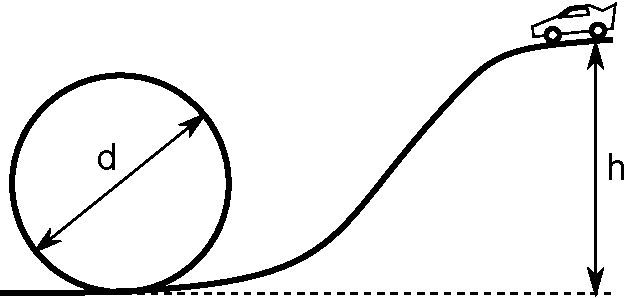
\includegraphics[width=\linewidth]{2012-v2g-05-silmus}%
\end{wrapfigure}
Mudelauto rada on kujutatud joonisel: auto alustab kaldtee tipus seisvast
asendist, kogub laskumisel kiirust ja teeb silmuses surmasõlme. Mis on
minimaalne kõrgus $h$, et auto silmuse läbimisel alla ei kukuks? Silmuse
läbimõõt on $d$. Hõõrdumisega arvestada ei ole vaja.
\fi


\ifHint
Autole mõjuvad raskusjõud ja tee toereaktsioon. Silmuses püsimiseks ei tohi toereaktsioon kaduda. Kriitiline olukord tekib silmuse ülemises punktis, sest siis on auto kiirus vähim ning raskusjõud tõmbab autot maksimaalselt teest eemale.
\fi


\ifSolution
Autole mõjuvad raskusjõud ja tee toereaktsioon. Silmuses püsimiseks ei tohi
toereaktsioon kaduda. Nende jõudude resultandi silmuse keskele
suunatud komponent moodustab kesktõmbejõu. Selle suurus sõltub auto kiirusest:
\[F_c=m\frac{v^2}{R},\]
kus $R$ on silmuse raadius.
Kriitiline olukord tekib silmuse ülemises punktis, kus auto kiirus on vähim ja
raskusjõud tõmbab autot risti teest eemale. Piirjuhul seal
toereaktsioon puudub ning raskusjõud on ise kesktõmbejõud:
\[ mg=\frac{mv^2}{d/2},\]
kus $m$ on auto mass ja $v$ kiirus.
Energia jäävuse seaduse kohaselt on auto kõrgus ja kiirus otseselt seotud:
\[ mgh'=\frac{mv^2}{2},\]
kus $h'$ on algpunkti ja uuritava punkti kõrguste vahe. Saadud võrrandit 
eelmisega läbi jagades saame vajaliku kõrguste erinevuse algpunkti ja silmuse 
haripunkti vahel:
\[ h'=\frac{d}{4}.\]
Otsitud kogukõrgus on silmuse läbimõõdu võrra suurem ja
\[ h=h'+d=1,25d.\;\]
\fi


\ifEngStatement
% Problem name: Loop-the-loop track
\begin{wrapfigure}{r}{42mm}%
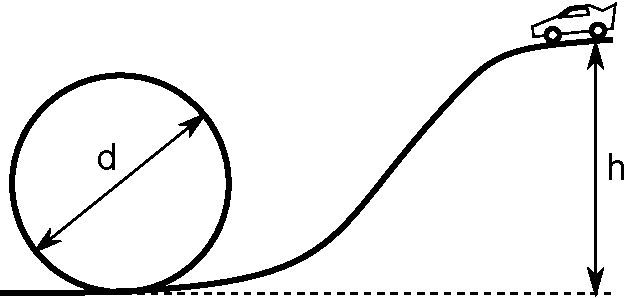
\includegraphics[width=\linewidth]{2012-v2g-05-silmus}%
\end{wrapfigure}
A toy car’s track is shown in the figure. The car begins from a resting position on top of the inclined track. The car accelerates while driving down and finally drives through a loop. What is the minimal height $h$ so that the car will not drop down while driving through the loop? The loop’s diameter is $d$. Do not account for friction.
\fi


\ifEngHint
Gravity force and normal force are applied to the car. To stay in the loop the normal reaction must not disappear. The critical situation is at the upper point of the loop because then the car’s speed is the smallest and the gravity force pulls the car maximally away from the road.
\fi


\ifEngSolution
The car is affected by gravity force and normal force of the track. To stay in the loop the normal force must not disappear. The component of the resultant of these forces which is directed to the center of the loop forms the centrifugal force. Its value depends on the car’s velocity:
\[F_c=m\frac{v^2}{R},\] 
where $R$ is the loop’s radius. Critical situation occurs in the upper point of the loop where the car’s velocity is the smallest and the gravity force pulls the car perpendicularly away from the track. At limit case there is no normal force and the gravity force itself is the centrifugal force:
\[ mg=\frac{mv^2}{d/2},\] 
where $m$ is the car’s mass and $v$ velocity. According to the conservation of energy the car’s height and velocity are directly related:
\[ mgh'=\frac{mv^2}{2},\]
where $h'$ is the difference between the heights of the initial point and the observed point. Dividing this equation by the previous one we get the necessary difference of heights between the initial point and the upper point of the loop:
\[ h'=\frac{d}{4}.\]
The desired total height is bigger by the diameter of the loop and
\[ h=h'+d=1,25d.\;\]
\fi
}